\documentclass[12pt,a4paper]{article}

% Language setting
\usepackage[british]{babel}

% Set page size and margins
\usepackage[a4paper,top=2cm,bottom=2cm,left=2.5cm,right=2.5cm,marginparwidth=1.75cm]{geometry}

%----------- APA style references & citations (starting) ---
% Useful packages
%\usepackage[natbibapa]{apacite} % APA-style citations.

\usepackage[style=apa, backend=biber]{biblatex} % APA 7th edition style citations using biblatex
\addbibresource{references.bib} % Your .bib file

% Formatting DOI in APA-7 style
%\renewcommand{\doiprefix}{https://doi.org/}

% Add additional APA 7th edition requirements
\DeclareLanguageMapping{british}{british-apa} % Set language mapping
\DeclareFieldFormat[article]{volume}{\apanum{#1}} % Format volume number

% Modify 'and' to '&' in the bibliography
\renewcommand*{\finalnamedelim}{%
  \ifnumgreater{\value{liststop}}{2}{\finalandcomma}{}%
  \addspace\&\space}
  
%----------- APA style references & citations (ending) ---


\usepackage{amsmath}
\usepackage{graphicx}
\usepackage[colorlinks=true, allcolors=blue]{hyperref}
\usepackage{hyperref}
%\usepackage{orcidlink}
\usepackage[title]{appendix}
\usepackage{mathrsfs}
\usepackage{amsfonts}
\usepackage{booktabs} % For \toprule, \midrule, \botrule
\usepackage{threeparttable} % For table footnotes
\usepackage{algorithm}
\usepackage{algorithmicx}
\usepackage{algpseudocode}
\usepackage{listings}
\usepackage{enumitem}
\usepackage{chngcntr}
\usepackage{booktabs}
\usepackage{lipsum}
\usepackage{subcaption}
\usepackage{authblk}
\usepackage[T1]{fontenc}    % Font encoding
\usepackage{csquotes}       % Include csquotes
\usepackage{diagbox}
\usepackage{comment}
\usepackage{url}

%\usepackage[justification=raggedright, singlelinecheck=false]{caption}
\usepackage{helvet}  % Load Helvetica (Arial-like)
\usepackage{lmodern}  % Ensures default LaTeX font is available

% label format: capital, centering, and parens
\renewcommand{\thesubfigure}{\Alph{subfigure}}

% Customize line spacing
\usepackage{setspace}
\onehalfspacing % 1.5 line spacing

% Redefine section and subsection numbering format
\usepackage{titlesec}
\titleformat{\section} % Redefine section numbering format
  {\normalfont\Large\bfseries}{\thesection.}{1em}{}
  
% Customize line numbering format to right-align line numbers
%\usepackage{lineno} % Add the lineno package
%\renewcommand\linenumberfont{\normalfont\scriptsize\sffamily\color{blue}}
%\rightlinenumbers % Right-align line numbers

%\linenumbers % Enable line numbering

% Define a new command for the fourth-level title.
\newcommand{\subsubsubsection}[1]{%
  \vspace{\baselineskip}% Add some space
  \noindent\textbf{#1\\}\quad% Adjust formatting as needed
}
% Change the position of the table caption above the table
\usepackage{float}   % for customizing caption position
\usepackage{caption}
\captionsetup[table]{position=top} % caption position for tables
\captionsetup[table]{labelfont=bf} % caption label
\captionsetup[figure]{labelfont=bf} % caption label

% Define the unnumbered list
\makeatletter
\newenvironment{unlist}{%
  \begin{list}{}{%
    \setlength{\labelwidth}{0pt}%
    \setlength{\labelsep}{0pt}%
    \setlength{\leftmargin}{2em}%
    \setlength{\itemindent}{-2em}%
    \setlength{\topsep}{\medskipamount}%
    \setlength{\itemsep}{3pt}%
  }%
}{%
  \end{list}%
}
\makeatother

% Suppress the warning about \@parboxrestore
\pdfsuppresswarningpagegroup=1

\date{}  % Remove date


\begin{document}


%----------


\begin{center}
{\Huge Article title article title article title}
\\[5ex]

{\large First Author} \\
{\small
Department, University, Street, City, State ZIP, Country \\
first.author@univ.edu \\
\url{https://orcid.org/0000-0002-1010-2288}
} \\[1.2em]

{\large Second MidName Author} \\
{\small
Department, Company, Street, City, State ZIP, Country \\
second.author@company.com
} \\[1.2em]

{\large Third Author} \\
{\small
Department, Organization, Street, City, State ZIP, Country \\
Department, University, Street, City, State ZIP, Country \\
third.author@org.org \\
\url{https://orcid.org/0000-0001-1015-3377}
} \\[1.2em]

{\large Fourth Author} \\
{\small
Department, Institute, Street, City, State ZIP, Country \\
fourth.author@inst.edu
} \\[1.2em]

{\large Fifth Author \small(Corresponding Author)} \\
{\small
Department, University, Street, City, State ZIP, Country \\
user\_id@univ.edu \\
\url{https://orcid.org/0000-0003-1025-5678}
}
\end{center}

\begin{abstract}
  Complete-aircraft boundary representation (B-Rep) models in Standard for the Exchange of Product model data (STEP) format contain numerous rivets and surface-feature instances, whose reliable recognition is challenged by class imbalance and costly background false positives. The framework represents B-Rep faces as graph nodes and integrates face geometric attributes, adjacency topology, and edge attributes for classification. 
  A dual-specialist GNN (graph neural network) employs independent encoders, classification heads, and decision thresholds for rivets and surface-feature, before fusing the outputs into background, rivet, and surface-feature classes. Training and testing are partitioned by complete aircraft rather than by randomly selected faces, preventing adjacent faces from the same aircraft from appearing in different datasets. The evaluation protocol focuses on per-aircraft errors, 
  background false positives, and maximum false-positive area. The original STEP face-id associated with each prediction is retained during subsequent rivet or surface-feature removal and host-face reconstruction, thereby supporting auditable downstream geometric processing. For large smooth shells, a smooth-shell guard is designed to reduce high-risk background misclassification. The framework supports traceable small-feature recognition and subsequent geometric processing for complete-aircraft B-Rep models,
   while per-aircraft evaluation is used to examine error characteristics and risk boundaries across different models.
%\lipsum[1]
\end{abstract}

\textbf{Keywords}: B-Rep,STEP traceability,graph learning,rivet recognition, surface features, geometric processing.  

%-------------------------------------------
% Paper Body
%-------------------------------------------
%--- Section ---%
\section*{Nomenclature}

\begin{tabbing}
$T$\qquad \= Temperature (K)\\
$u_i$ \> Velocity in the x-direction (m/s)\\
$\tau_{ij}$ \> Shear stress (N/m2)\\
$\omega$ \> Specific turbulent dissipation rate (1/s)\\
$Y_\omega$ \> Dissipation of $\omega$
\end{tabbing}



%--- Section ---%
\section{Introduction}

Your introduction goes here! Simply start writing your document and use the Recompile button to view the updated PDF preview. Examples of commonly used commands and features are listed below to help you get started.
\lipsum[2]

Once familiar with the editor, you can find various project settings in the Overleaf menu, accessed via the button at the top left of the editor. To view tutorials, user guides, and further documentation, please visit our \href{https://www.overleaf.com/learn}{help library}, or head to our plans page to \href{https://www.overleaf.com/user/subscription/plans}{choose your plan}. 

This is an example of a new paragraph with a numbered footnote\footnote{\url{https://data.gov.uk/}} and a second footnote marker.\footnote{Example of footnote text.}


%--- Section ---%
\section{Related Work and Problem Formulation}\label{sec2}

Building on the motivation for recognising small surface features in complete-aircraft STEP models, this section establishes the relevant background and formulates the problem addressed in this work. STEP/B-Rep models encode both geometric entities and their topological relationships; faces, edges, and face adjacency therefore provide a direct basis for face-level analysis \parencite{iso10303_42_2025}. Earlier CAD feature-recognition studies predominantly relied on attributed adjacency graphs, geometric rules, volumetric decomposition, and hint-based reasoning to identify local structures with manufacturing semantics \parencite{han2000manufacturing,shah2001discourse}. More recent work has explored learning directly from B-Rep parameterisations and topology, treating face-level prediction as a graph-learning problem and thereby avoiding some geometric and correspondence losses associated with intermediate mesh or point-cloud representations \parencite{jayaraman2021uvnet,lambourne2021brepnet,wu2024aagnet}.

Complete aircraft differ materially from the mechanical parts commonly considered in public CAD-learning studies. They may contain many faces, extensive continuous curved surfaces, topology that is partitioned by modelling and exchange operations, and substantial variation in external shape, component organisation, and face decomposition across aircraft. Rivets, decals, windows, and related small surface features are often much less prevalent than background faces, while their local geometry can be similar to that of smooth fuselage or shell regions. Such class imbalance can cause learning and evaluation to be dominated by the majority class \parencite{he2009learning}. Moreover, a false positive on a large background face is not merely a face-level error: when predictions drive feature removal and host-face reconstruction, it can introduce an avoidable downstream geometric-processing risk. Evaluation should therefore consider this risk in addition to aggregate face-level correctness.

Existing public studies have largely addressed machining features or modelling-operation semantics in mechanical parts, and some formulations jointly consider semantic segmentation, instance grouping, and process-related relations \parencite{lambourne2021brepnet,wu2024aagnet}. Systematic discussion of small surface-feature recognition in complete-aircraft STEP models remains limited. A random face-level train--test split may also place strongly related faces from the same aircraft on both sides of the partition, leading to an optimistic estimate of cross-model generalisation; the distribution of related samples across evaluation partitions is a recognised source of leakage risk in machine-learning studies \parencite{kapoor2023leakage}. In addition, published evaluations commonly focus on segmentation labels or intermediate representations, whereas a traceable evidence chain from predictions to the corresponding STEP face-id is not yet a standard evaluation constraint. Therefore, it is necessary to define the face-level three-class task, specify model-level evaluation constraints, and develop a method that retains face-id traceability for subsequent geometric processing.


\subsection{Face-Level Feature Recognition in STEP/B-Rep Models}

The STEP standard supports the representation of three-dimensional solids using boundary representations (B-Reps), in which topological entities such as vertices, edges, and faces are associated with geometric entities including points, curves, and surfaces. Their connectivity is further expressed through structures such as loops and shells \parencite{iso10303_42_2025}. A face in a STEP model is therefore not an isolated geometric patch: it carries geometric information, such as surface type, area, normal direction, and parameter domain, while also belonging to a topological structure formed through shared edges. Face-level representations provide a traceable unit for subsequent geometric processing, feature localisation, visual annotation, and engineering analysis. They also preserve the correspondence between a prediction and the original B-Rep entity, avoiding sole reliance on meshed or point-cloud approximations that may weaken this correspondence \parencite{jayaraman2021uvnet,lambourne2021brepnet}.

Traditional CAD feature-recognition methods have primarily supported computer-aided process planning and the extraction of manufacturing information. Representative approaches include graph matching, heuristic geometric reasoning, volumetric decomposition and recomposition, and hint-based reasoning \parencite{han2000manufacturing,shah2001discourse}. Rule-based methods commonly identify features such as holes, slots, and bosses by combining predefined geometric thresholds, surface types, concavity or convexity, boundary conditions, and local topological templates. Attributed adjacency graph methods encode faces and their adjacency relations as an attributed graph, and then locate candidate features through subgraph matching or pattern recognition \parencite{babic2008review,han2000manufacturing}. These methods are interpretable and effective when feature definitions, geometric constraints, and topological patterns are well specified. However, feature interactions, domain dependence, multiple valid interpretations, and complex surface geometry increase the difficulty of rule construction and matching \parencite{shah2001discourse}. Consequently, maintaining rule sets, transferring thresholds, and preserving robustness across models can become challenging for models with continuous free-form surfaces, complex local connections, and varying face partitions.

More recently, learning-based B-Rep methods have provided an alternative to explicit rule matching. A B-Rep can be represented as a graph in which faces serve as nodes, shared-edge or adjacency relations serve as edges, and face geometry, edge attributes, and local topology are encoded as node or edge features \parencite{colligan2022hierarchical,jayaraman2021uvnet}. In this representation, graph neural networks can aggregate information from adjacent faces and progressively incorporate a wider topological context, framing face-level classification as node classification on a graph \parencite{lambourne2021brepnet}. UV-Net combines geometric information from the parametric domains of surfaces and curves with adjacency-graph topology, whereas BRepNet performs topological message passing over faces, edges, and oriented coedges \parencite{jayaraman2021uvnet,lambourne2021brepnet}. For machining feature recognition, Hierarchical CADNet similarly encodes face adjacency, surface geometry, and edge convexity to predict a feature class for each B-Rep face \parencite{colligan2022hierarchical}.

Nevertheless, representative studies have largely considered mechanical CAD models, synthetic B-Rep samples, or machining-feature data, where the semantic classes are commonly associated with modelling operations or manufacturing features such as holes, slots, and bosses \parencite{colligan2022hierarchical,jayaraman2021uvnet,lambourne2021brepnet}. The complete-aircraft STEP models considered in this work instead involve an aircraft-scale setting, a high proportion of continuous free-form surfaces, complex structural hierarchy, and substantial variation in face decomposition and feature distribution across aircraft. Rivets often correspond to small and densely distributed local face sets, while surface features may span different scales and curvature regions; both must be distinguished from large, smooth background regions. These differences indicate that face-level small-feature recognition on complete-aircraft B-Rep graphs, particularly for rivets and surface features, warrants further systematic investigation.

Accordingly, existing studies do not directly resolve the three-class face-level task considered here, namely assigning every original B-Rep face to \textit{background}, \textit{rivet}, or \textit{surface-feature}. The task requires not only generalisation across complete aircraft and aircraft types, but also stable traceability from predictions to the original STEP face-id for human review, visual annotation, and downstream engineering workflows. In addition, falsely labelling a large smooth background face as a feature may create a material engineering risk; aggregate classification measures alone are therefore insufficient to characterise recognition quality. The next subsection discusses the specific challenges of small surface-feature recognition in complete-aircraft models.

\subsection{Challenges and Problem Formulation for Small Surface-Feature Recognition}\label{subsec1}

Small surface-feature recognition in complete-aircraft STEP models is not solely a face-level classification problem. It is jointly constrained by class distribution, geometric and topological variation, cross-aircraft generalisation, and the engineering consequences of downstream geometric processing. The following subsections define these challenges and formulate the task considered in this work.

\subsubsection{Class Imbalance and Scale Variation}\label{subsubsec:class_imbalance}

Small surface-feature recognition in complete-aircraft STEP models first faces pronounced scale and class imbalance. Compared with background faces that constitute the main body of the fuselage, wings, and engine nacelles, rivets usually correspond to only a small number of local faces with limited area. The \textit{surface-feature} class may include windows, decals, and other surface-attached structures, whose geometric scale, shape, and spatial distribution are more variable. Consequently, background faces commonly dominate both face count and surface coverage; model training and aggregate evaluation can therefore be dominated by the majority class, while missed detections and false detections of minority classes may be obscured by overall accuracy. This is consistent with the general challenge in imbalanced learning, where the majority class can dominate the decision boundary and reduce recognition of minority classes \parencite{he2009learning}.

\subsubsection{Free-Form Surfaces and B-Rep Face-Partition Variation}\label{subsubsec:brep_variation}

The continuous free-form surfaces of complete aircraft mean that the geometric boundary between a small feature and its background is not always explicit. A rivet may appear as a local protrusion, a depression, or a small structure composed of multiple adjacent faces, whereas a \textit{surface-feature} may have planar, curved, or mixed boundary forms. In addition, different STEP exporters, modelling histories, and Boolean operations can alter the face partition of a similar local structure, producing variation in face count, adjacency pattern, and surface parameterisation. It is therefore difficult to reliably distinguish a true feature from local geometric variation on a fuselage or wing using only the area, surface type, or curvature of an individual face. Recognition must instead consider face adjacency, local topological context, and a wider structural context.

\subsubsection{Cross-Aircraft Generalisation, Traceability, and Engineering Risk}\label{subsubsec:generalisation_traceability}

Generalisation across complete aircraft is an important constraint of this task. If training and test sets are split randomly by individual faces or local subgraphs, geometrically similar and topologically related faces from the same aircraft may occur in both partitions. Test results may then partly reflect reproduction of already observed whole-aircraft structures rather than generalisation to unseen aircraft. Machine-learning research has shown that dependence between training and test samples can lead to data leakage and overly optimistic performance estimates \parencite{kapoor2023leakage}. Accordingly, this work uses the complete aircraft as the basic unit of data partitioning: training and test aircraft are independent at the model level, so that evaluation better reflects the intended use on unseen complete-aircraft models.

The task output is intended not only for semantic annotation but also for subsequent geometric processing and human review. Each prediction should remain traceable to its original STEP face-id, enabling the corresponding face to be located, visualised, and verified on the original B-Rep. False positives on large smooth background faces require particular attention. If such a face is incorrectly labelled as a \textit{rivet} or \textit{surface-feature} and subsequently participates in feature removal, host-face reconstruction, or other geometric operations, it may have a disproportionate effect on downstream model integrity. Therefore, in addition to conventional face-level classification metrics, evaluation should examine background faces incorrectly identified as features for each aircraft and the areas of the affected faces, so as to more fully characterise the engineering risk of the recognition result.

\subsection{Limitations of Existing Methods and Research Gaps}\label{subsec:research_gaps}

Existing B-Rep learning studies have established the feasibility of face-level prediction from geometric and topological information. BRepNet performs topological message passing over faces, edges, and oriented coedges for modelling-operation segmentation, while Hierarchical CADNet combines B-Rep face adjacency, surface geometry, and edge attributes for machining-feature recognition \parencite{lambourne2021brepnet,colligan2022hierarchical}. These studies provide relevant methodological foundations, but their label systems and evaluation objectives are not identical to the task considered in this work.

Published B-Rep learning benchmarks primarily use modelling-operation labels or machining-feature classes. They do not directly define the three-class task of distinguishing \textit{background}, \textit{rivet}, and \textit{surface-feature} faces in complete-aircraft STEP models \parencite{lambourne2021brepnet,colligan2022hierarchical}. In particular, existing evidence does not establish whether a unified classifier or separately trained predictors is more suitable for the two target feature categories. The dual-specialist GNN in this work is therefore treated as a testable architectural choice rather than as a consequence already demonstrated by prior studies. Its value must be assessed through a controlled comparison with a unified three-class model under the same data split and training budget.

Evaluation protocols also require careful alignment with the intended deployment setting. If related samples are shared between training and test partitions, the resulting evaluation may provide an overly optimistic estimate of performance on independent objects. For the present task, the complete aircraft is consequently used as the unit of data partitioning, so that the evaluation addresses transfer to unseen aircraft rather than recognition of related faces from an already observed model.

In addition, existing studies commonly evaluate semantic segmentation or machining-feature labels at the face level. The present workflow requires each prediction to remain linked to the corresponding original STEP face-id, because the output is subsequently used for feature removal and host-face reconstruction. Face-level classification scores alone do not establish this geometry-processing traceability. Retaining the original face-id therefore forms an explicit output constraint in this work and provides an auditable link from the predicted label to the B-Rep entity used in subsequent operations.

These considerations define the scope of the proposed method: the dual-specialist GNN tests task-specific prediction design, aircraft-level partitioning supports an evaluation aligned with the intended use case, and face-id retention connects face-level predictions to subsequent geometric processing. The following subsection formalises the corresponding graph representation and classification task.

\subsection{Face-Level Three-Class Problem Formulation}\label{subsec:problem_formulation}

Accordingly, each complete-aircraft STEP model is represented as a face-level graph $G=(V,E)$, where the node set $V$ corresponds to original B-Rep faces and the edge set $E$ represents face adjacency. Nodes and edges carry attributes derived from faces, edges, and their local topology. For each node $v_i$, the objective is to predict a class label $y_i \in \{\textit{background}, \textit{rivet}, \textit{surface-feature}\}$ while preserving a one-to-one correspondence between the prediction and the original STEP face-id. This formulation jointly incorporates cross-aircraft generalisation, three-class face-level recognition, prediction traceability, and the risk of false positives on large background faces, thereby establishing the basis for the subsequent method design and evaluation protocol.

\subsection{Overview of the Proposed Method and Contributions}\label{subsec:method_overview}

To address the recognition, geometric simplification, and simulation-acceleration requirements associated with small surface features in complete-aircraft STEP/B-Rep models, this work proposes a face-level graph-learning framework that integrates cross-aircraft generalisation, engineering-risk control, and geometric traceability. Each complete aircraft is represented as a B-Rep face graph whose nodes are faces and whose edges encode topological adjacency; face geometric attributes, topological relations, and edge attributes are incorporated as input information. Beyond semantic recognition, the framework is intended to support the location and removal of non-critical small features, thereby reducing unnecessary mesh complexity and supporting more efficient simulation preparation and numerical analysis.

The main contributions of this work are as follows:
\begin{enumerate}[label=(\arabic*)]
  \item A face-level B-Rep graph representation is constructed for three-class prediction: \textit{background}, \textit{rivet}, and \textit{surface-feature}. The \textit{surface-feature} class encompasses non-rivet small surface features, including decals and windows.
  \item A dual-specialist GNN architecture is developed, comprising a rivet specialist and a surface-feature specialist. The two specialists learn the respective discrimination patterns of the target feature categories, and their predictions are fused at the final stage.
  \item Training and testing are partitioned by complete aircraft rather than by randomly selected faces. In addition to conventional classification measures, the evaluation considers, for each aircraft, the number of background faces falsely identified as features and the maximum area of a falsely identified background face. These risk-oriented measures address the engineering consequence of misclassifying large smooth shell faces.
  \item The original STEP face-id is retained for every prediction, allowing the predicted label to be traced back to a specific geometric entity. This traceability supports subsequent feature removal, host-face localisation, and host-face reconstruction, and provides an entity-level basis for geometric simplification.
  \item A protection mechanism is introduced for large smooth shell background faces to reduce the risk of high-impact background misclassification. It is intended to preserve critical exterior geometry during feature processing while supporting mesh-count reduction and simulation acceleration.
\end{enumerate}

The next section presents the face-level graph construction, node and edge features, dual-specialist GNN, data partitioning and training procedure, prediction fusion, smooth-shell protection mechanism, and the geometry-traceability and feature-processing workflow for simulation-oriented mesh simplification.


%--- Section ---%
\section{Example of first level head}\label{sec3}

\subsection{This is an example of second level head - subsection head}\label{subsec2}

\subsubsection{This is an example of third level head - subsubsection head}\label{subsubsec2}
\lipsum[8]

\subsubsubsection{This is an example of fourth level head - paragraph head}
\lipsum[9]


%--- Section ---%
\section{How to include equations}\label{sec4}

Equations in \LaTeX{} can either be inline or set as display equations. For
inline equations use the \verb+$...$+ commands. Eg: the equation
$H\psi = E \psi$ is written via the command \verb+$H \psi = E \psi$+.

For display equations (with auto generated equation numbers)
one can use the equation or eqnarray environments:
\begin{equation}
\|\tilde{X}(k)\|^2 \leq\frac{\sum\limits_{i=1}^{p}\left\|\tilde{Y}_i(k)\right\|^2+\sum\limits_{j=1}^{q}\left\|\tilde{Z}_j(k)\right\|^2 }{p+q},
\label{eq1}
\end{equation}
where
\begin{align}
D_\mu &=  \partial_\mu - ig \frac{\lambda^a}{2} A^a_\mu \nonumber \\
F^a_{\mu\nu} &= \partial_\mu A^a_\nu - \partial_\nu A^a_\mu + g f^{abc} A^b_\mu A^a_\nu
\label{eq2}
\end{align}
Notice the use of \verb+\nonumber+ in the align environment at the end
of each line, except the last, so as not to produce equation numbers on
lines where no equation numbers are required. The \verb+\label{}+ command
should only be used at the last line of an align environment where
\verb+\nonumber+ is not used.
\begin{equation}
Y_\infty = \left( \frac{m}{\textrm{GeV}} \right)^{-3}
    \left[ 1 + \frac{3 \ln(m/\textrm{GeV})}{15}
    + \frac{\ln(c_2/5)}{15} \right]
\label{eq3}
\end{equation}
The class file also supports the use of \verb+\mathbb{}+, \verb+\mathscr{}+ and
\verb+\mathcal{}+ commands. As such \verb+\mathbb{R}+, \verb+\mathscr{R}+
and \verb+\mathcal{R}+ produces $\mathbb{R}$, $\mathscr{R}$ and $\mathcal{R}$
respectively 
%(refer Subsubsection~\ref{subsubsec3}).

Equations must be provided as editable text, either in a Word or LaTeX source file. They should be numbered consecutively through the manuscript as shown in Equations \ref{eq1}, \ref{eq2} and \ref{eq3}. In APA style, when discussing numbered equations in the text, write out the word “Equation” and give the number. For example, you would write “see Equation \ref{eq1}.”
Use no punctuation after the equation if it appears at the end of a sentence; however, it is permissible (and may even be necessary) to place some form of punctuation after it (a comma or semi-colon, for example) if it appears in the middle of the sentence and is followed by text. In any case, maintain the coherence of all sentences with equations in them.


%--- Section ---%
\section{How to include tables}\label{sec5}

Use the table and tabular environments for basic tables --- see Tables~\ref{tab1} and \ref{tab2}, for example. Table \ref{tab1} is an sample figure including table footnotes. For more information, please see this help article on \href{https://www.overleaf.com/learn/latex/tables}{tables}. 

\begin{table}[!ht]
\caption{Sample table with footnotes\label{tab1}}
\begin{threeparttable}
\begin{tabular*}{\columnwidth}{@{\extracolsep\fill}llll@{\extracolsep\fill}}
\toprule
column 1 & column 2 & column 3 & column 4\\
\midrule
row 1 & data 1 & data 2 & data 3 \\
row 2 & data 4 & data 5\tnote{1} & data 6 \\
row 3 & data 7 & data 8 & data 9\tnote{2} \\
\bottomrule
\end{tabular*}
\begin{tablenotes}
\item Source: This is an example of table footnote. This is an example of table footnote. This is an example of table footnote. This is an example of table footnote. This is an example of table footnote.
\item[1] Example of a first table footnote.
\item[2] Example of a second table footnote.
\end{tablenotes}
\end{threeparttable}
\end{table}

\begin{table*}[!ht]
\caption{Example of a lengthy table which is set to full textwidth.\label{tab2}}
\tabcolsep=0pt
\begin{threeparttable}
\begin{tabular*}{\textwidth}{@{\extracolsep{\fill}}lcccccc@{\extracolsep{\fill}}}
\toprule
& \multicolumn{3}{c}{Element 1\tnote{1}} & \multicolumn{3}{c}{Element 2\tnote{2}} \\
\cmidrule(lr){2-4}\cmidrule(lr){5-7}
Project & Energy & $\sigma_{\mathrm{calc}}$ & $\sigma_{\mathrm{expt}}$ & Energy & $\sigma_{\mathrm{calc}}$ & $\sigma_{\mathrm{expt}}$ \\
\midrule
Element 3 & 990 A & 1168 & $1547\pm12$ & 780 A & 1166 & $1239\pm100$ \\
Element 4 & 500 A & 961 & $922\pm10$ & 900 A & 1268 & $1092\pm40$ \\
\bottomrule
\end{tabular*}
\begin{tablenotes}
\item Note: This is an example of table footnote this is an example of table footnote this is an example of table footnote this is an example of~table footnote this is an example of table footnote.
\item[1] Example of a first table footnote.
\item[2] Example of a second table footnote.
\end{tablenotes}
\end{threeparttable}
\end{table*}


%--- Section ---%
\section{How to include figures}\label{sec6}

\subsection{Figures}

Figures must be inserted directly into the main text of the manuscript and should not be placed collectively at the end. All figures must be cited in the main text in numerical order, and each figure should be placed immediately after the paragraph in which it is first mentioned.

All figures must be presented in a size and format that ensure clear readability. Each figure must be accompanied by an appropriate caption or legend. Figures should be numbered consecutively throughout the manuscript using Arabic numerals (for example, Figure 1, Figure 2, and Figure 3). For figures appearing in an appendix, the numbering should be prefixed with the appendix letter (for example, Figure A1 and Figure B1).

Authors are strongly encouraged to use two-dimensional (2D) graphics rather than three-dimensional (3D) graphics unless a 3D representation is essential, as 2D graphics are generally clearer, more accurate, and easier to interpret. Border lines around figures should be removed. Authors should also avoid the use of white text and background colors in figures, as these may reduce legibility.

When referring to figures in the manuscript text and in figure captions, authors must use the full term “Figure” rather than the abbreviation “Fig.”

Note that your figure will automatically be placed in the most appropriate place for it, given the surrounding text and taking into account other figures or tables that may be close by. You can find out more about adding images to your documents in this help article on \href{https://www.overleaf.com/learn/how-to/Including_images_on_Overleaf}{including images on Overleaf}.



\begin{figure}[!ht]
\centering

\includegraphics[width=0.5\linewidth]{figures/cat_momo_1.png}
\caption{\label{fig:cat1}This cat picture is located at the 'figures' folder.}
\end{figure}


If a figure consists of multiple subfigures as shown in Figure 2, each subfigure should be identified by a capital letter, such as (A), (B), (C), and so forth, centered below the corresponding subfigure. Authors should follow the style illustrated in Figure 2 of the manuscript template. Subfigure labels must not be embedded within the image itself.

When citing a figure that contains multiple subfigures in the main text, authors should use the format Figure 2A, Figure 2B, and so on. In the figure caption, the corresponding descriptions should be given using the format (A), (B), (C), etc.

When multiple images are combined into a single figure using a grid arrangement, authors should ensure that the layout does not compromise visibility. In particular, placing too many images in a single horizontal row may reduce the size of each image and make textual or graphical details difficult to read. Where necessary, authors should reduce the number of images arranged horizontally. For example, if a 2 × 4 layout results in images that are too small, a 4 × 2 layout may provide better visibility.


\begin{figure}[!ht]
    \centering
    \begin{subfigure}{0.45\textwidth}
        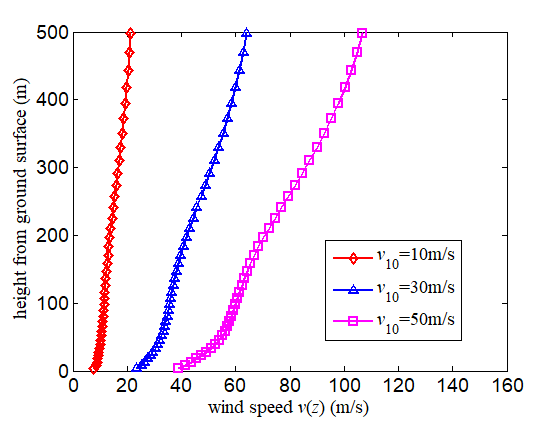
\includegraphics[width=\linewidth]{figures/fig_a.png}
        \caption{}
    \end{subfigure}
    \hfill
    \begin{subfigure}{0.45\textwidth}
        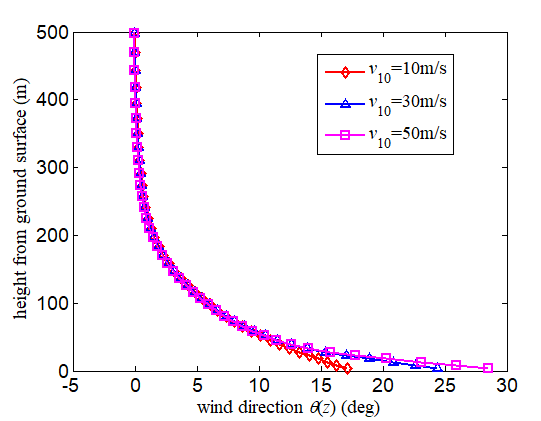
\includegraphics[width=\linewidth]{figures/fig_b.png}
        \caption{}
    \end{subfigure}
    \vskip\baselineskip
    \begin{subfigure}{0.45\textwidth}
        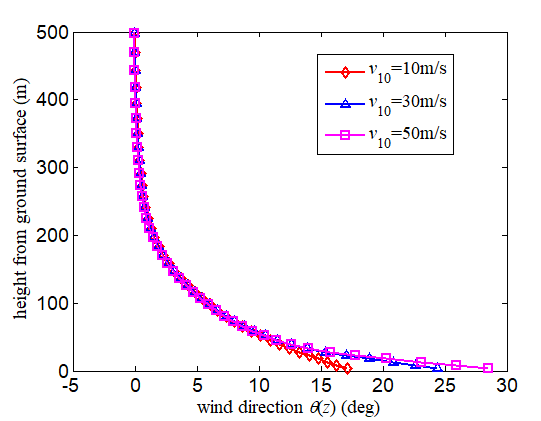
\includegraphics[width=\linewidth]{figures/fig_c.png}
        \caption{}
    \end{subfigure}
    \hfill
    \begin{subfigure}{0.45\textwidth}
        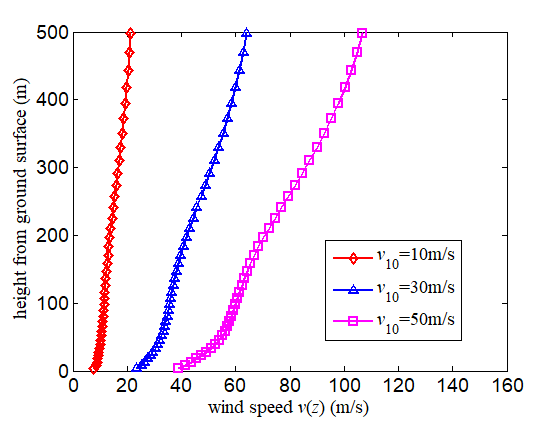
\includegraphics[width=\linewidth]{figures/fig_a.png} % 첫 번째 그림 다시 사용
        \caption{}
    \end{subfigure}
    \caption{Overall caption for the four figures. (A) Caption for figure A. (B) Caption for figure B. (C) Caption for figure C. (D) Caption for figure D.}
    \label{fig:multi_figs}
\end{figure}

\subsection{Alt text}

Incorporating alt text (alternative text) when submitting your paper helps to foster inclusivity and accessibility. Well-written alt text enables readers with visual impairments, including those using screen readers, to understand the content and context of your figures. The purpose of alt text is to provide concise, informative descriptions of the essential information conveyed by each figure so that all readers have equitable access to the same information and can engage with the visual elements integral to scholarly content. Including alt text demonstrates a commitment to accessibility and can enhance the overall impact and reach of your work. Although some journals include alt text below each figure caption, as shown in Figure \ref{fig:alt_text}, for administrative convenience we ask authors to submit a separate MS Word file containing a list of all alt texts once the manuscript has been accepted.
Please note the following points regarding alt text:
\begin{itemize}
\item Alt text applies to all images, figures, illustrations, and photographs.
\item Alt text is primarily accessed via assistive technologies (e.g., screen readers) and may not appear in the typeset article.
\item Once the manuscript has been accepted, please submit alt text in a separate MS Word file.
\item \href{https://static.primary.prod.gcms.the-infra.com/static/site/journals/document/alt-text-figure-accessibility.pdf?node=1329505d4d63d87a12ed}{Detailed guidance on how to draft and submit alt text.}
\end{itemize}


\begin{figure}[!ht]
\centering
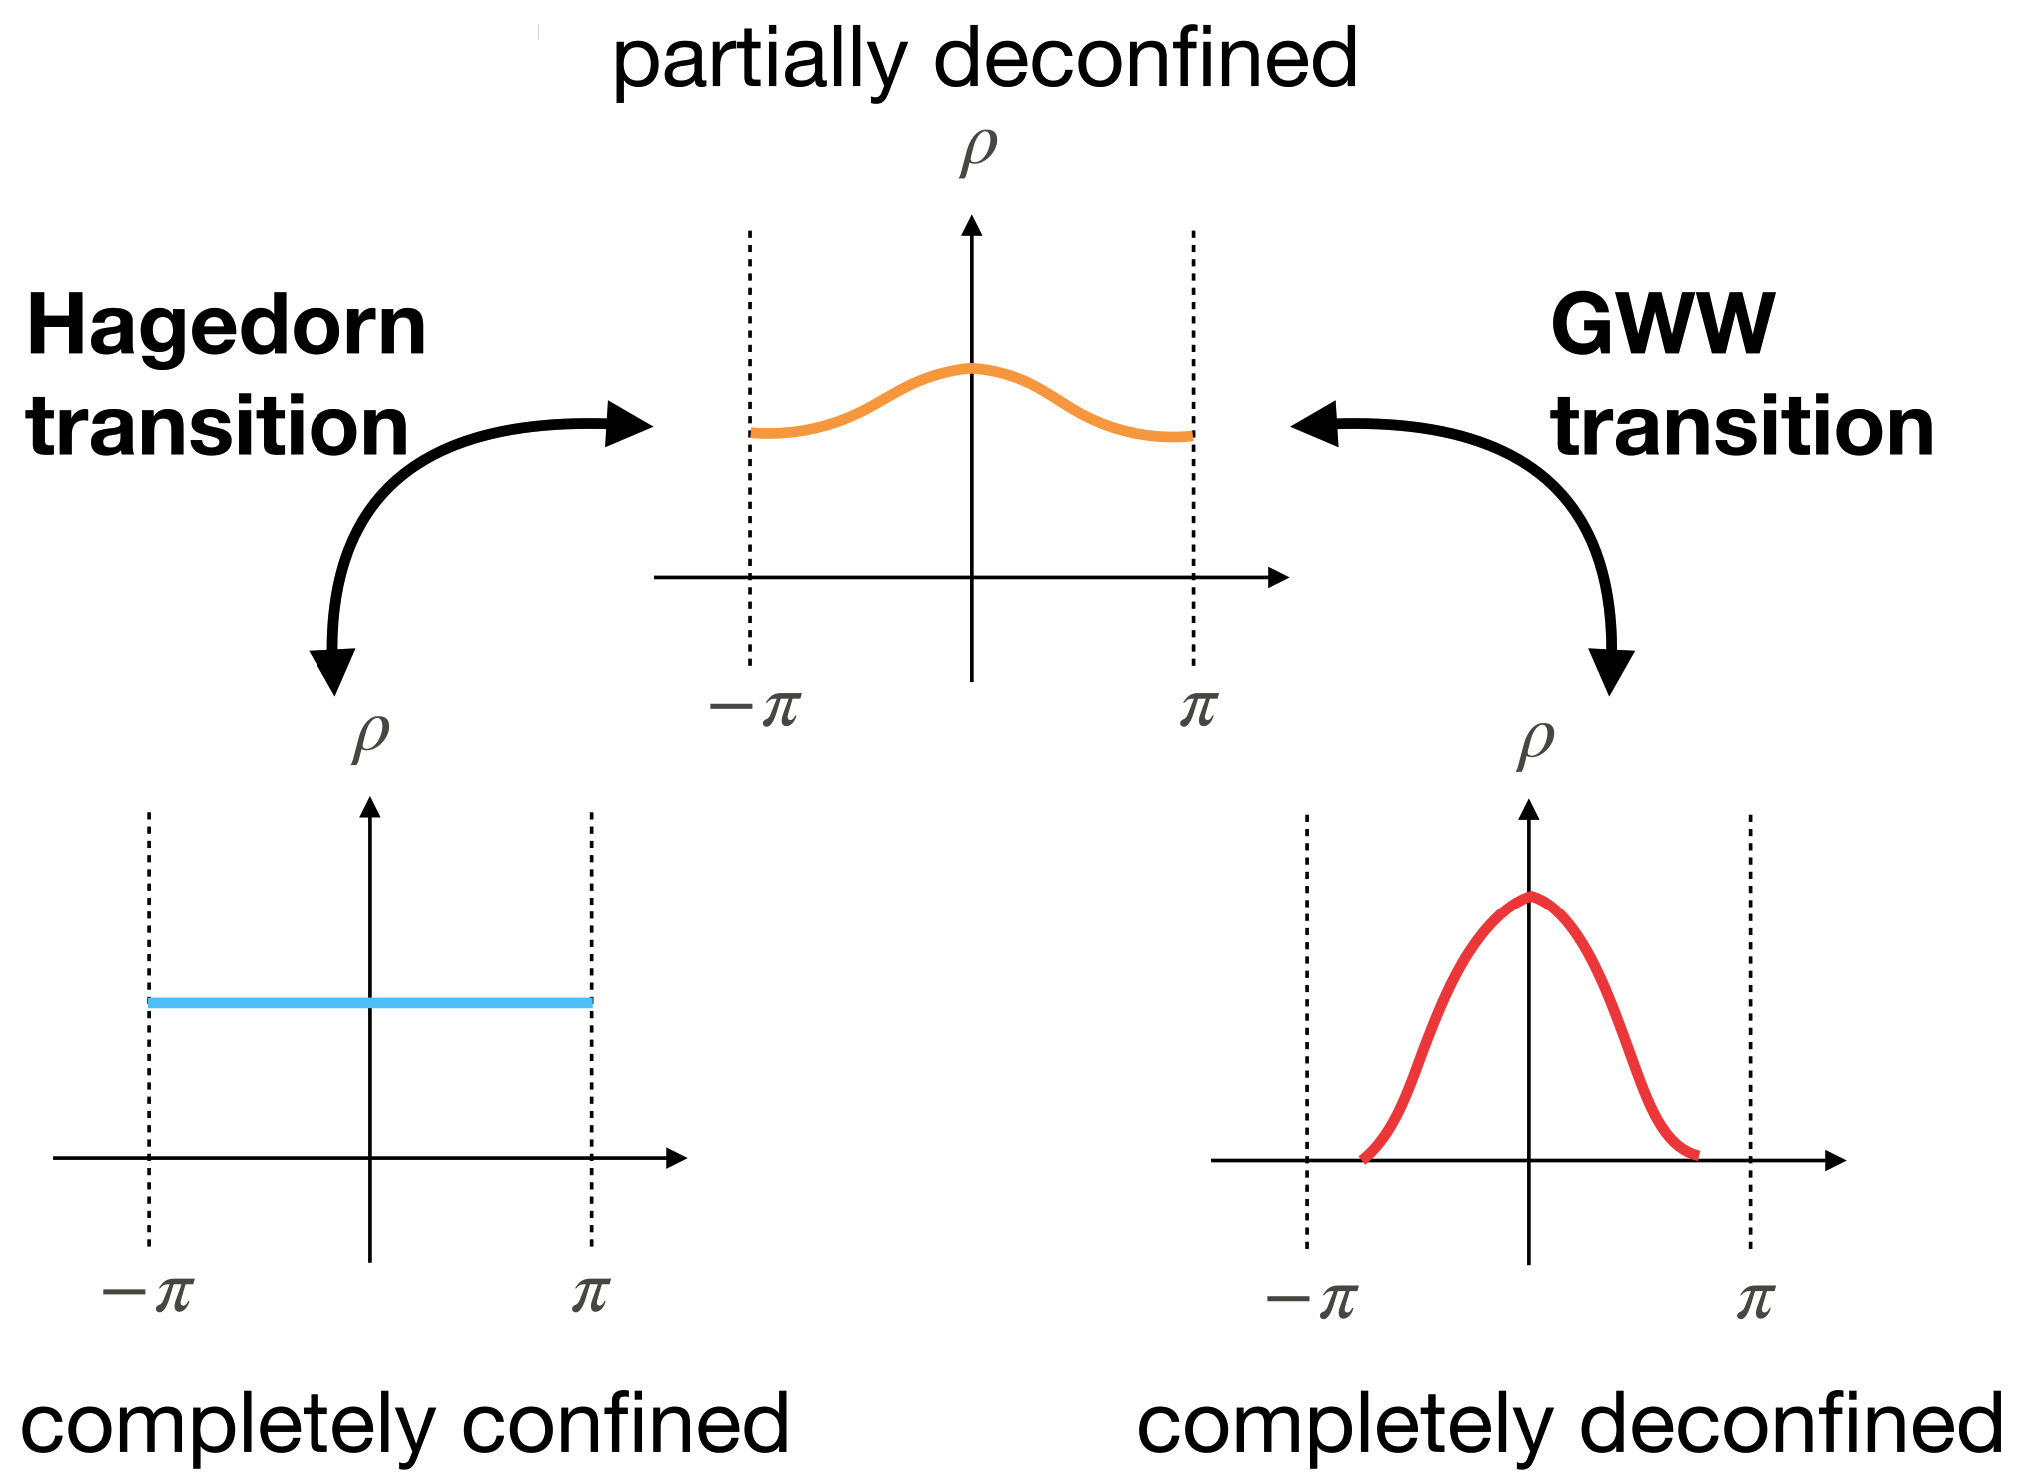
\includegraphics[width=0.7\linewidth]{figures/alt_text_example.png}
\caption{\label{fig:alt_text}Completely confined, partially deconfined, and completely deconfined phases correspond to uniform, nonuniform but jointed, and disjointed distributions of Polyakov line phases, respectively.\\
\textbf{Alt Text:} Graphical representation of three phases—completely confined, partially deconfined, and completely deconfined—depicting Polyakov line phases with corresponding transition profiles.
}
\end{figure}

%--- Section ---%
\section{How to include algorithms, program codes, and listings}\label{sec8}
Packages \verb+algorithm+, \verb+algorithmicx+, and \verb+algpseudocode+ are used for setting algorithms in latex.
For this, one has to use the below format:

\begin{verbatim}
\begin{algorithm}
\caption{<alg-caption>}\label{<alg-label>}
\begin{algorithmic}[1]
. . .
\end{algorithmic}
\end{algorithm}
\end{verbatim}

You may need to refer to the above-listed package documentation for more details before setting an \verb+algorithm+ environment.
To set program codes, one has to use the \verb+program+ package. We need to use the \verb+\begin{program}+ \verb+...+
\verb+\end{program}+ environment to set program codes.

\begin{algorithm}[!ht]
\caption{Calculate $y = x^n$}\label{algo1}
\begin{algorithmic}[1]
\Require $n \geq 0 \vee x \neq 0$
\Ensure $y = x^n$
\State $y \Leftarrow 1$
\If{$n < 0$}
        \State $X \Leftarrow 1 / x$
        \State $N \Leftarrow -n$
\Else
        \State $X \Leftarrow x$
        \State $N \Leftarrow n$
\EndIf
\While{$N \neq 0$}
        \If{$N$ is even}
            \State $X \Leftarrow X \times X$
            \State $N \Leftarrow N / 2$
        \Else[$N$ is odd]
            \State $y \Leftarrow y \times X$
            \State $N \Leftarrow N - 1$
        \EndIf
\EndWhile
\end{algorithmic}
\end{algorithm}

Similarly, for \verb+listings+, one has to use the \verb+listings+ package. To set environments similar to the \verb+verbatim+ environment, the \verb+\begin{lstlisting}+ \verb+... + \verb+\end{lstlisting}+ environment is used . Refer to the \verb+lstlisting+ package documentation for more details on this.

\begin{minipage}{\hsize}%
\lstset{language=Pascal}% Set your language (you can change the language for each code-block optionally)
\begin{lstlisting}[frame=single,framexleftmargin=-1pt,framexrightmargin=-17pt,framesep=12pt,linewidth=0.95\textwidth]
for i:=maxint to 0 do
begin
{ do nothing }
end;
Write('Case insensitive ');
Write('Pascal keywords.');
\end{lstlisting}
\end{minipage}


%--- Section ---%
\section{How to include lists}\label{sec7}

List in \LaTeX{} can be of three types: numbered, bulleted, and unnumbered. The ``enumerate'' environment produces a numbered list, the 
``itemize'' environment produces a bulleted list, and the ``unlist''
environment produces an unnumbered list.
In each environment, a new entry is added via the \verb+\item+ command.

\begin{enumerate}[label=\arabic*.]
\item This is the 1st item
\item Enumerate creates numbered lists, itemize creates bulleted lists, and unnumerate creates unnumbered lists.

\begin{enumerate}[label=\alph*.]
\item Second level numbered list. Enumerate creates numbered lists, itemize creates bulleted lists, and description creates unnumbered lists.
\item Second level numbered list. Enumerate creates numbered lists, itemize creates bulleted lists, and description creates unnumbered lists.

\begin{enumerate}[label=(\roman*)]
\item Third level numbered list. Enumerate creates numbered lists, itemize creates bulleted lists, and description creates unnumbered lists.
\item Third level numbered list. Enumerate creates numbered lists.
\end{enumerate}

\item Second level numbered list. Enumerate creates numbered lists, itemize creates bulleted lists, and description creates unnumbered lists.
\end{enumerate}

\item Numbered lists continue.
\end{enumerate}
Lists in \LaTeX{} can be of three types: enumerate, itemize, and description.
In each environment, a new entry is added via the \verb+\item+ command.

\begin{itemize}
\item First level bulleted list. This is the 1st item
\item First level bulleted list. Itemize creates bulleted lists, and description creates unnumbered lists.

\begin{itemize}
\item Second level dashed list. Itemize creates bulleted lists, and description creates unnumbered lists.
\item Second level dashed list. Itemize creates bulleted lists, and description creates unnumbered lists.
\end{itemize}

\item First level bulleted list. Bullet lists continue.
\end{itemize}

\noindent
Example of unnumbered list items:

\begin{unlist}
\item Sample unnumberd list text. Sample unnumberd list text. Sample unnumberd list text. Sample unnumberd list text. Sample unnumberd list text.

\item Sample unnumberd list text. Sample unnumberd list text. Sample unnumberd list text.

\item Sample unnumberd list text. Sample unnumberd list text. Sample unnumberd list text. Sample unnumberd list text. 
\end{unlist}


%--- Section ---%
\section{How to add citations and a references list}

The references used in this manuscript are maintained in \verb|references.bib| and cited in the text with the template's author--year commands.



If you have an \href{https://www.overleaf.com/user/subscription/plans}{upgraded account}, you can also import your Mendeley or Zotero library directly as a \verb|.bib| file, via the upload menu in the file-tree.

\subsection{Citation in text}
Please ensure that every reference cited in the text is also present in the reference list (and vice versa). Citations in the text should follow the referencing style used by the American Psychological Association. You are referred to the Publication Manual of the American Psychological Association (APA), Seventh Edition, ISBN 978-1-4338-3215-4, copies of which may be ordered online. References in the Abstract should be avoided, but if essential, then cite the author(s) and year(s). Unpublished results and personal communications are not recommended in the reference list but may be mentioned in the text. If these references are included in the reference list, they should follow the standard reference style of the journal and should include a substitution of the publication date with either ‘Unpublished results’ or ‘Personal communication’. The citation of a reference as ‘in press’ implies that the item has been accepted for publication. 

An APA in-text citation includes only three items: the last name(s) of the author(s), the year the source was published, and sometimes the page or location of the information. More than one reference from the same author(s) in the same year must be identified by the letters ‘a’, ‘b’, ‘c’, etc., placed after the year of publication. The following paragraph shows examples of APA style of citations.





\subsection{References}
The Reference Section, also called the Reference List or Cited Works List, is a list of the full-text details of the in-text citations that have been used in the main text. It includes information such as the name of the author(s), the year the source was published, the full title of the source, and the URL or page range. The Reference Section allows the reader to find the text easily and can be considered as the long-hand format of the in-text citation. It is found at the end of the piece of writing. The works in a reference section should be arranged first alphabetically and then further sorted chronologically if necessary.

\subsubsection{Web references}
As a minimum, the full URL and the date when the reference was last accessed should be given. Any further information, if known (DOI, author names, dates, reference to a source publication, etc.), should also be given. Web references can be listed separately (e.g., after the reference list) under a different heading if desired or can be included in the reference list. With standard numerical .bst files, only numerical citations are possible. With an author-year .bst file, both numerical and author-year citations are possible. 

\subsubsection{Examples of reference style}
You can find information about the examples of APA-style references to various sources at the following site:\\
\url{https://apastyle.apa.org/style-grammar-guidelines/references/examples}.


%--- Section ---%
\section{Conclusions}
Some conclusions here.

%-------------------------------------------
% Acknowledgement Sections
%-------------------------------------------

%--- Mandatory Section ---%
\section*{Conflicts of interest} 
The authors must declare conflicts of interest or state “The authors declare no conflict of interest.” Authors must identify and declare any personal circumstances or interests that may be perceived as inappropriately influencing the representation or interpretation of reported research results. A detailed definition of conflicts of interest is available at the following site: \url{https://academic.oup.com/journals/pages/authors/preparing_your_manuscript/ethics#conflict}.

%--- Mandatory Section ---%
\section*{Author contributions}
The authors must specify the individual contributions of all authors, identified by full names, according to NISO CrediT (Contributer Roles Taxonomy) described at the following site: \url{https://credit.niso.org/}. An example statement is as follows:

\noindent\textbf{Kunwoo Lee}: Conceptualization, Methodology, Software. \textbf{Shuming Gao}: Data curation, Writing—original draft. \textbf{Sang Hun Lee}: Visualization, Investigation. \textbf{Jami J. Shah}: Supervision. \textbf{Hiromasa Suzuki}: Software, Validation. \textbf{Myung-Il Roh}: Writing—review \& editing.

%--- Section ---%
\section*{Funding}
Cite all funding for your research, providing the grant number and the funder name. An example statement is as follows: This work is supported in part by funds from the National Science Foundation (NSF: \# 1636933 and \# 1920920). 

If the funder is listed in the Crossref funder registry (\url{https://www.crossref.org/services/funder-registry/}), the funder name should appear exactly as it does in that database. Where grants were received by specific members of the author group, they should be identified by initials. 

More information on funding agency requirements is available at  \url{https://academic.oup.com/pages/open-research/open-access/complying-with-funder-policies}.

%--- Section ---%
\section*{Data availability}
The data availability statement should provide information on where and under what conditions the data directly supporting the publication can be accessed. Sample data availability statements are available at the following site: \url{https://academic.oup.com/pages/open-research/research-data#Data%20Availability%20Statements}.

%--- Section ---%
\section*{Acknowledgments}
The authors thank those people or institutions that have helped you in the preparation of the manuscript. 


%-------------------------------------------
% References
%-------------------------------------------

% Print bibliography
\printbibliography




%-------------------------------------------
% Appendix
%-------------------------------------------
% Activate the appendix in the doc
% from here on sections are numerated with capital letters 
%\appendix

% Change equation numbering format to be sequential within sections in the appendix
\renewcommand\theequation{\Alph{section}\arabic{equation}} % Redefine equation numbering format
\counterwithin*{equation}{section} % Number equations within sections
\renewcommand\thefigure{\Alph{section}\arabic{figure}} % Redefine equation numbering format
\counterwithin*{figure}{section} % Number equations within sections
\renewcommand\thetable{\Alph{section}\arabic{table}} % Redefine equation numbering format
\counterwithin*{table}{section} % Number equations within sections



\begin{appendices}


%--- For single section ---%
%\section*{Appendix}

%--- For multiple sections ---%
% Appendix formatting
\renewcommand{\thesection}{Appendix \Alph{section}}
\renewcommand{\thesubsection}{\Alph{section}.\arabic{subsection}}

%--- Section ---%
\section{Section title of first appendix}
Appendices are used for supplementary material that is relevant to the main text but not essential for inclusion in the text itself—for example, questionnaires, interview transcripts, extended data tables, or equipment descriptions.
\begin{itemize}
\item If there is only one appendix, label it as “Appendix”; if there are multiple appendices, label them as “Appendix A,” “Appendix B,” and so on, arranging them in the order they appear in the paper. 
\item All appendices must be referenced in the main text, and only items that enhance the reader’s understanding or support your argument should be included.
\item Tables and figures in an appendix should be labeled separately (e.g., Table \ref{tab_a1}, Figure \ref{fig:cat2}).
\end{itemize}

%--- Subsection ---%
\subsection{Fist subsection title of first appendix}
As shown in Equation \ref{eq_a1}, the section number is inserted in the equation number.
\lipsum[11]

\begin{equation}
Y_\infty = \left( \frac{m}{\textrm{GeV}} \right)^{-3}
    \left[ 1 + \frac{3 \ln(m/\textrm{GeV})}{15}
    + \frac{\ln(c_2/5)}{15} \right]
\label{eq_a1}
\end{equation}

%--- Subsection ---%
\subsection{Second subsection title of first appendix}
As shown in Table \ref{tab_a1}, the section number is inserted in the table number.

\begin{table}[!ht]
\caption{Sample table with three parts and five columns\label{tab_a1}}
\begin{threeparttable}
\begin{tabular*}{\columnwidth}{@{\extracolsep\fill}lllll@{\extracolsep\fill}}
\toprule
column 1 & column 2 & column 3 & column 4 & column 5\\
\midrule
row 1 & data 0 & data 1 & data 2 & data 3 \\
row 2 & data 4 & data 5 & data 6 & data 7 \\
row 3 & data 8 & data 9 & data 10 & data 11\\
\bottomrule
\end{tabular*}
\end{threeparttable}
\end{table}

%--- Subsubsection ---%
\subsubsection {Subsubsection title of first appendix}
\lipsum[12]


%--- Section ---%
\section{Section title of second appendix}

As shown in Figure \ref{fig:cat2}, the section number is inserted in the figure number.
\lipsum[13]

% figure b1
\begin{figure}[!htbp]
\centering
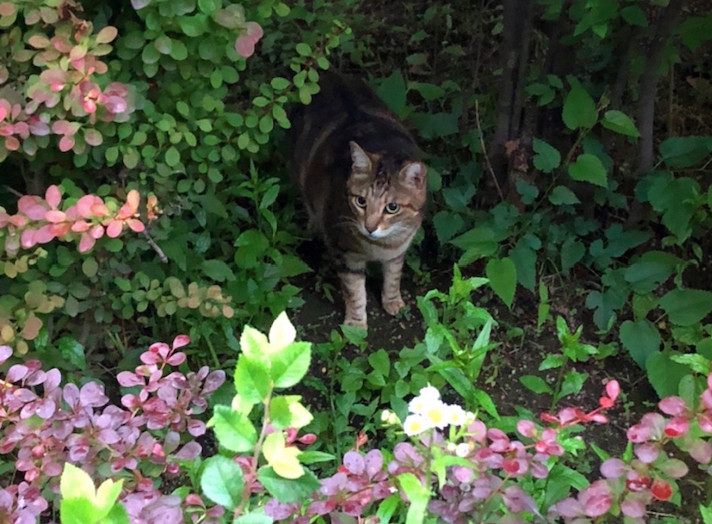
\includegraphics[width=0.8\linewidth]{figures/cat_momo_2.jpg}
\caption{\label{fig:cat2}This cat picture is located at the 'figures' folder.}
\end{figure}

\lipsum[14]

\subsection{Appendix subsection title here}
\lipsum[15]

\end{appendices}

\end{document}
